\documentclass[12pt]{article}
\usepackage{setspace,graphicx,amsmath,geometry,fontspec,titlesec,soul,bm,subfigure}
\titleformat{\section}[block]{\LARGE\bfseries}{\arabic{section}}{1em}{}[]
\titleformat{\subsection}[block]{\Large\bfseries\mdseries}{\arabic{section}.\arabic{subsection}}{1em}{}[]
\titleformat{\subsubsection}[block]{\normalsize\bfseries}{\arabic{subsection}-\alph{subsubsection}}{1em}{}[]
\titleformat{\paragraph}[block]{\small\bfseries}{[\arabic{paragraph}]}{1em}{}[]
\setmainfont{Times New Roman}
\renewcommand{\baselinestretch}{1.15}
\renewcommand\contentsname{Inhaltverzeichnis}
\geometry{a4paper,left=2.5cm,right=2.5cm,top=2.5cm,bottom=2.5cm}
\begin{document}
	\newpagestyle{main}{            
		\sethead{Ziqing Yu}{Übung 1}{3218051}     
		\setfoot{}{\thepage}{}     
		\headrule                                     
		\footrule                                       
	}
	\pagestyle{main}
\tableofcontents
\newpage
\section{Einleitung}
In dieser Übung führt man 3 unterschiedliche Ausgleichungsverfahren mit Panda durch. Die Beobachtungen sind vorgegeben. Die Qualität und Güte werden diskutiert und beurteilt. 

\section{Teilspurminimierung}
\begin{figure}[ht]\centering
	\subfigure[Fehlerellipse]{
		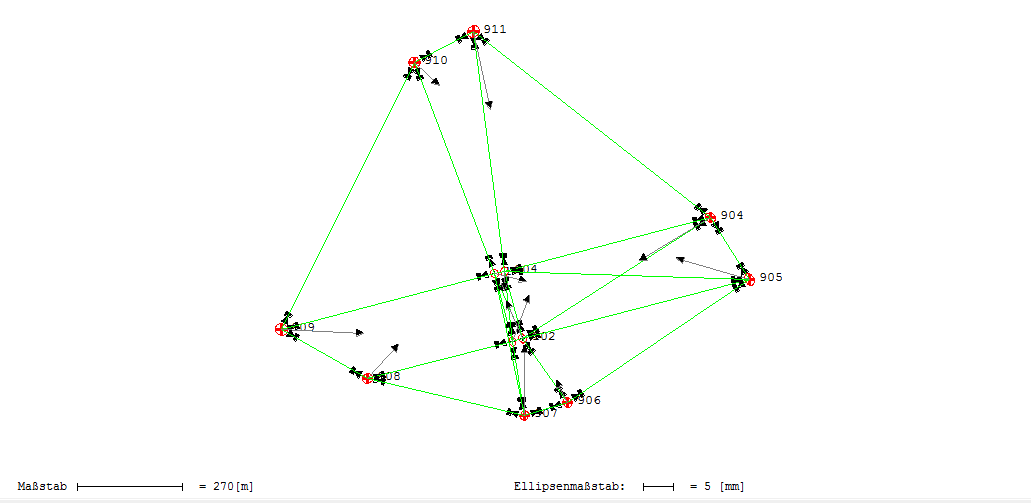
\includegraphics[width=0.9\textwidth]{1-Fehler.png}}
	\subfigure[Konfidenzellipse]{
		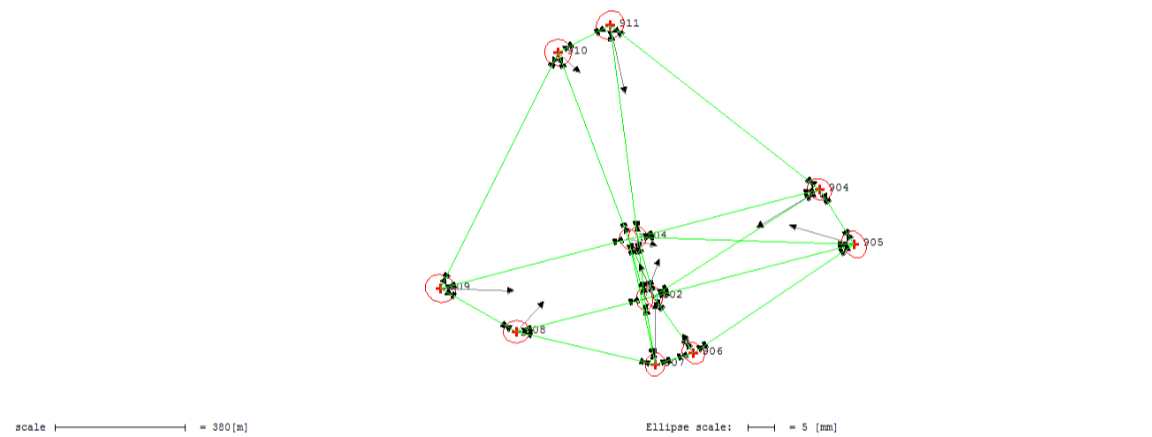
\includegraphics[width=0.9\textwidth]{1-Konfidenz.png}}
	\caption{Stützpunkte als Datumspunkte}
\end{figure}
\newpage

\section{Gesamtspurminimierung}
\begin{figure}[ht]\centering
	\subfigure[Fehlerellipse]{
		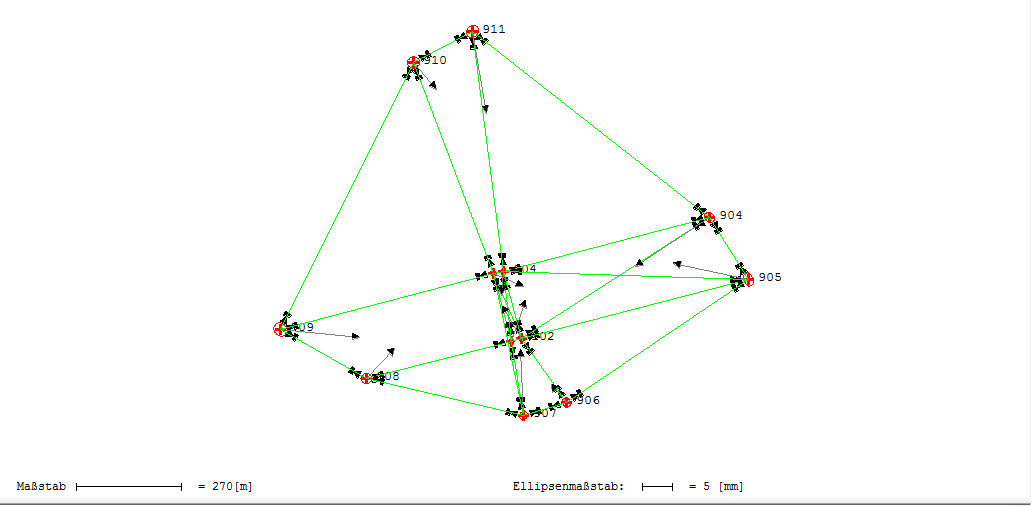
\includegraphics[width=0.9\textwidth]{2-Fehler.png}}
	\subfigure[Konfidenzellipse]{
		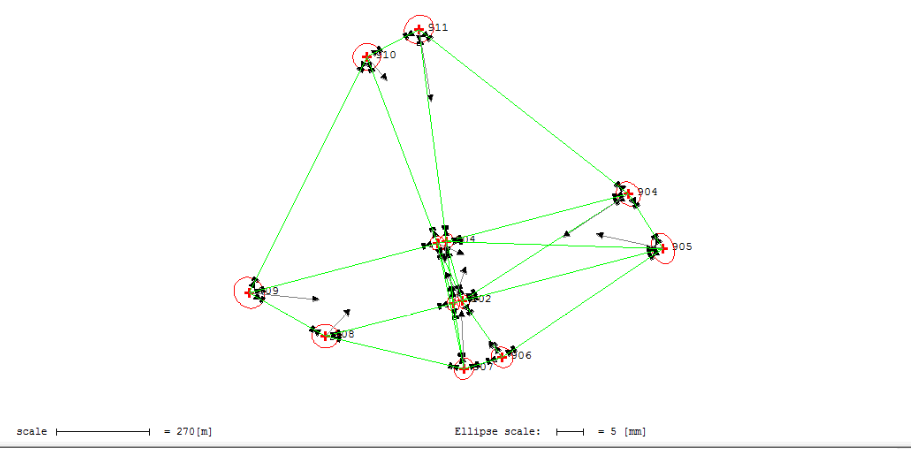
\includegraphics[width=0.9\textwidth]{2-Konfidenz.png}}
	\caption{Alle Punkte als Datumspunkte}
\end{figure}
\newpage

\section{Ausgleichung unter Zwang}
\begin{figure}[ht]\centering
	\subfigure[Fehlerellipse]{
		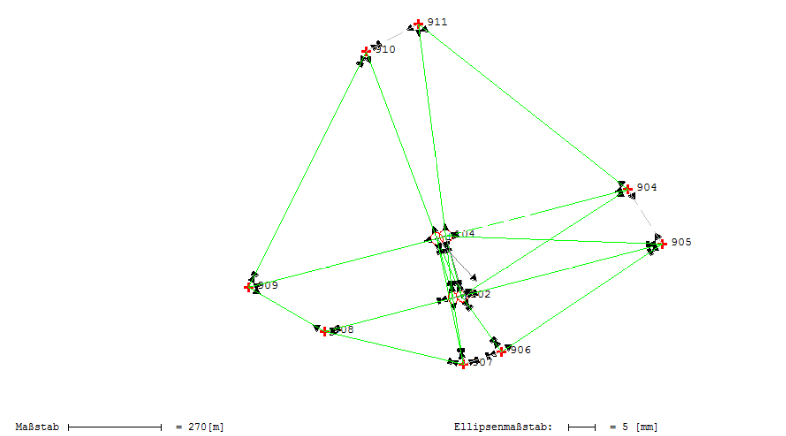
\includegraphics[width=0.9\textwidth]{3-Fehler.png}}
	\subfigure[Konfidenzellipse]{
		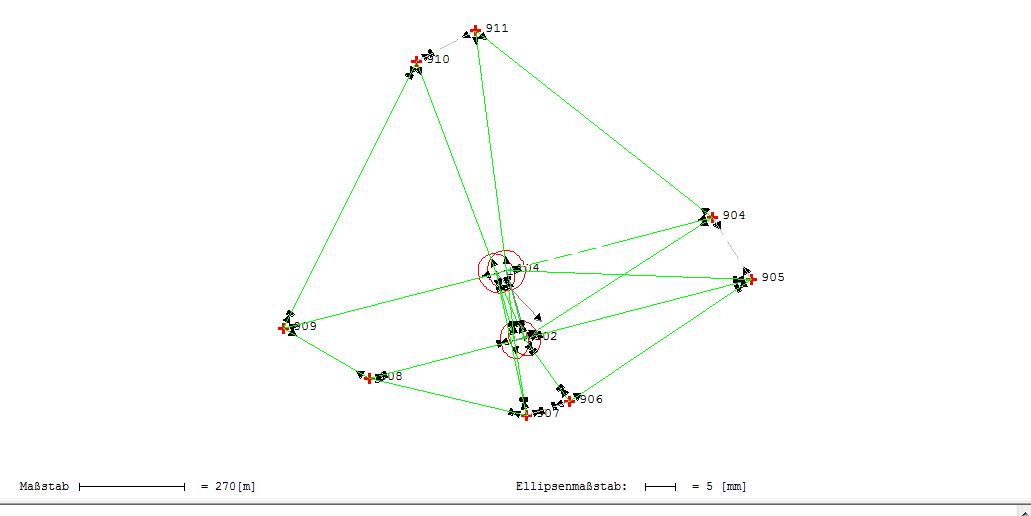
\includegraphics[width=0.9\textwidth]{3-Konfidenz.png}}
	\caption{Ausgleichung unter Zwang}
\end{figure}
\newpage

\section{HELMERT'schen Punktfehler}
HELMERT'schen-Punktfehler \newline
\begin{equation*}
\sigma_{P}=\sqrt{\sigma_{x}^2 + \sigma_{y}^2}
\end{equation*}
\begin{figure}[ht] \centering
\begin{tabular}{llll}
	\hline
	\multicolumn{1}{|l|}{Punktenummer} & \multicolumn{1}{l|}{$\sigma_x \ (mm)$}    & \multicolumn{1}{l|}{$\sigma_y \ (mm)$}    & \multicolumn{1}{l|}{$\sigma_P \ (mm)$}      \\ \hline
	\multicolumn{1}{|l|}{101}          & \multicolumn{1}{l|}{0,69} & \multicolumn{1}{l|}{0,51} & \multicolumn{1}{l|}{0,8580} \\ \hline
	\multicolumn{1}{|l|}{102}          & \multicolumn{1}{l|}{0,65} & \multicolumn{1}{l|}{0,55} & \multicolumn{1}{l|}{0,8515} \\ \hline
	\multicolumn{1}{|l|}{103}          & \multicolumn{1}{l|}{0,64} & \multicolumn{1}{l|}{0,58} & \multicolumn{1}{l|}{0,8637} \\ \hline
	\multicolumn{1}{|l|}{104}          & \multicolumn{1}{l|}{0,66} & \multicolumn{1}{l|}{0,57} & \multicolumn{1}{l|}{0,8721} \\ \hline
	\multicolumn{1}{|l|}{904}          & \multicolumn{1}{l|}{0,68} & \multicolumn{1}{l|}{0,75} & \multicolumn{1}{l|}{1,0124} \\ \hline
	\multicolumn{1}{|l|}{905}          & \multicolumn{1}{l|}{0,84} & \multicolumn{1}{l|}{0,76} & \multicolumn{1}{l|}{1,1328} \\ \hline
	\multicolumn{1}{|l|}{906}          & \multicolumn{1}{l|}{0,67} & \multicolumn{1}{l|}{0,70} & \multicolumn{1}{l|}{0,9690} \\ \hline
	\multicolumn{1}{|l|}{907}          & \multicolumn{1}{l|}{0,72} & \multicolumn{1}{l|}{0,62} & \multicolumn{1}{l|}{0,9502} \\ \hline
	\multicolumn{1}{|l|}{908}          & \multicolumn{1}{l|}{0,69} & \multicolumn{1}{l|}{0,81} & \multicolumn{1}{l|}{1,0640} \\ \hline
	\multicolumn{1}{|l|}{909}          & \multicolumn{1}{l|}{0,85} & \multicolumn{1}{l|}{0,93} & \multicolumn{1}{l|}{1,2599} \\ \hline
	\multicolumn{1}{|l|}{910}          & \multicolumn{1}{l|}{0,81} & \multicolumn{1}{l|}{0,83} & \multicolumn{1}{l|}{1,1597} \\ \hline
	\multicolumn{1}{|l|}{911}          & \multicolumn{1}{l|}{0,88} & \multicolumn{1}{l|}{0,86} & \multicolumn{1}{l|}{1,2304} \\ \hline
\end{tabular}
\end{figure}
\begin{itemize}
\item Der HELMERT'schen-Punktfehler beschreibt die Qualität bzw. die Messgenauigkeit eines Punktes. 
\item Die Fehlerellipse beschreibt die Größe der Fehlern in verschiedenen Richtungen. 
\item Die Konfindenzellepse beschreibt die möglichen Gebiete, wo der Punkt genau liegt. 
\end{itemize}
\newpage

\section{Qualität des Netzes mit Teilspurminimierung}
\begin{itemize}
\item Die lokale Genauigkeit lautet HELMERT'schen-Punktfehler. Da alle sind zwischen $0,8$ bis $1,3$ mm, ist die Messung ziemlich genau. 

\item Die globale Genauigkeit kann durch die Formel $ sp\sum_{xx}$ berechnet werden. $sp\sum_{xx}=1,2696 \cdot 10^{-5}$. D.h. die Messung hat eine gute Genauigkeit. 

\item Innere Zuverlässigkeit kann man durch $b = \frac{f}{n}$ berechnen, wobei $f$ ist die Freiheitsgrade und $n$ ist der Anzahl der Beobachtungen. Aus dem Protokoll ist $f = 67$ also $(100-36+3)$ und $n= 100$, deshalb ist Innere Zuverlässigkeit $b = 0,67$

\item Äußere Zuverlässigkeit $\Phi_{i}^{2} = (1-r_{i}´) \cdot p_{ii} \cdot \nabla l_{i}^2 $ wobei $r_i$ Teilredundanz und $p_{ii}$ Gewicht sind, $\nabla l_{i}$ wird hier direkt vom Protokoll gelesen. Zum Beispiel, bei der erste Beobachtung, $r_1 = 0,37$, $p_{11} = 1$, $\nabla l_{i}=  0,087mgon \cdot \frac{\pi}{200} = 1,367 \cdot 10^{-5}$ , $\Phi_{1}^{2} = 1.1766 \cdot 10^{-10}$
\end{itemize}

\section{Vergleichung}
Bei freier Ausgleichung werden alle Punkten ausgeglichen und bei Ausgleichung unter Zwang sind nur Stützpunkten bzw. Festpunkten ausgeglichen. 
\end{document}